\documentclass[12pt,a4paper]{extarticle}

\usepackage{packages}
\usepackage{environments}
\usepackage{commands}

\graphicspath{{./figures/}{../code/paper_icml/figures/}{../code/paper_neurips/figures/}{../../anova/lc_anova/results/figures/}}

\definecolor{darkblue}{RGB}{0,0,128}
\hypersetup{colorlinks=true, linkcolor=black, citecolor=blue, urlcolor=darkblue, bookmarks=true, hypertexnames=true}

\usepackage{titlepage}

\addbibresource{bibl.bib}

\renewcommand{\baselinestretch}{1.5}
\setlength{\parindent}{1.25cm}
\setlength{\parskip}{0pt}

\counterwithin{table}{section}
\counterwithin{figure}{section}
\counterwithin{equation}{section}

\renewcommand{\theenumi}{\arabic{enumi}}
\renewcommand{\labelenumi}{\arabic{enumi}.}
\renewcommand{\theenumii}{\arabic{enumi}.\arabic{enumii}}
\renewcommand{\labelenumii}{\arabic{enumi}.\arabic{enumii}.}
\renewcommand{\theenumiii}{\arabic{enumi}.\arabic{enumii}.\arabic{enumiii}}
\renewcommand{\labelenumiii}{\arabic{enumi}.\arabic{enumii}.\arabic{enumiii}.}

% ===== Title page parameters =====
\setTitle{Application of Physics-Informed Neural Networks for Modeling Liquid and Gas Flow in Porous Media}
\setTitleRu{Применение физически информированных нейронных сетей для моделирования течения жидкости и газа в пористой среде}
\setProjectType{Research Project}

\setStudent{Anna Alexandrovna Lazareva}
\setStudentGroup{БКНАД222}
\setStudentYear{4th year of study}
\setStudentDate{20.05.2026}

\setAdvisor{Tarakanov Alexander Aleksandrovich}
\setAdvisorDegree{PhD}
\setAdvisorTitle{Associate Professor}
\setAdvisorAffiliation{Faculty of Computer Science, HSE University}

\setYear{2026}

% ===================================================
\begin{document}

\makeTitlePage

\setcounter{page}{2}

{\hypersetup{linkcolor=black}
\renewcommand{\contentsname}{Contents}
\tableofcontents
}

\newpage

% ================================================================
\section*{Abstract}
\addcontentsline{toc}{section}{Abstract}

Physics-informed neural networks (PINNs) approximate solutions of PDEs by minimising a weighted combination of residual, boundary, initial, and (optional) data losses. Their performance is dominated by two choices that the practitioner must fix before training: the relative weights of the loss components, and the values of the physical parameters that enter the PDE. A poor weighting collapses the optimisation onto one constraint and ignores another; a different parameter value requires retraining the network from scratch. Both choices are normally addressed by grid search or by adaptive heuristics on top of grid search, which scales poorly across the parameter axis.

This thesis develops the \emph{loss-conditional PINN} (\LCPINN{})~--- a single network $u_\theta(x, \param)$ that takes the conditioning vector $\param$ as an explicit input alongside the spatial coordinates and is trained to satisfy a continuous family of PDE problems indexed by $\param$. Two regimes of conditioning are studied uniformly: $\param$ as the simplex of loss weights (for problems where loss balancing is the bottleneck, e.g.~viscous Burgers and Buckley--Leverett displacement in a porous medium), and $\param$ as a physical PDE parameter (wavenumber for parametric Helmholtz, harmonic-potential strength for parametric Schr\"{o}dinger). In the parametric regime, FiLM modulation~\cite{perez2018film} of the hidden activations combined with an L-BFGS refinement pass on a fixed quadrature support produces accuracy that is consistently within an order of magnitude of separately retrained baselines while amortising training across the whole parameter family.

The thesis reports the following empirical and theoretical results. For 1D Helmholtz over $k \in [1, 10]$, a single LC-PINN attains mean relative-$L^2$ error $9.39 \times 10^{-4}$ on a five-point evaluation grid, improving over SA-PINN~\cite{mcclenny2020sapinn} by $3.4\times$ and over ReLoBRaLo~\cite{bischof2021relobralo} by $4.1\times$ while requiring less total wall time than retraining all five PINNs. For Schr\"{o}dinger 1D, the LC-PINN reaches $1.99 \times 10^{-4}$ mean rel-$L^2$ across the harmonic-potential family, $20\times$ better than the per-$\alpha$ SA-PINN baseline on the grid mean. The 2D and 3D Helmholtz benchmarks extend without changing the core method. In the loss-weight regime, a single LC-PINN on viscous Burgers achieves $K=100$-shot averaged rel-$L^2 = 3.47 \times 10^{-3}$, matching the strongest single-shot baseline within a factor of two and outperforming the adaptive-weight baselines by more than an order of magnitude. On viscous-regularised Buckley--Leverett ($\varepsilon = 10^{-2}$), the porous-media application that motivates the thesis, the LC-PINN reaches rel-$L^2 = 1.03 \times 10^{-2}$ while SA-PINN saturates above $0.4$. A local optimisation analysis (Theorem~\ref{thm:loss-decay}) explains the consistent improvement in the parametric regime: the extra FiLM degrees of freedom enlarge the descent set in parameter space, yielding an instantaneous loss-decay rate at least as large as that of the standard PINN at the same effective parameter vector. A complementary $\lambda$-invariance result (Proposition~\ref{prop:lambda-invariance}) shows that global minimisers of the LC objective recover residual minimisers across the whole parameter family.

A short interpretability section applies a functional analysis-of-variance (ANOVA) decomposition to the trained 2D Helmholtz LC-PINN. The dominant subset is the three-way interaction $S_{xyk} = 0.43$, with bootstrap 95\,\% confidence interval $[0.41, 0.44]$. By ANOVA orthogonality, this implies an a-priori lower bound on the relative-$L^2$ error of any architecturally simpler solver: an additive solver $u(x, y, k) = f_{xy}(x, y) + f_k(k)$ has floor $\sqrt{S_{xk} + S_{yk} + S_{xyk}} \approx 0.76$; a pair-additive solver has floor $\sqrt{S_{xyk}} \approx 0.66$. We verify the predictions to within $0.002$ absolute against the exact analytic projection at $N = 10^6$ samples.

Source code, configuration files, and the LaTeX manuscript are released at \url{https://github.com/annalzrv/bachelor_thesis}.

\section*{Keywords}
\addcontentsline{toc}{section}{Keywords}

physics-informed neural networks; loss-conditional training; parametric partial differential equations; porous media flow; Buckley--Leverett displacement; FiLM conditioning; L-BFGS refinement; functional ANOVA decomposition; Sobol sensitivity indices.

\newpage

% ================================================================
\section*{Аннотация}
\addcontentsline{toc}{section}{Аннотация}

\selectlanguage{russian}

Физически информированные нейронные сети (PINN) приближают решения уравнений в частных производных (УЧП) минимизацией взвешенной комбинации остаточных, граничных, начальных и (опционально) дата-потерь. Эффективность метода определяется двумя выборами, которые делаются до обучения: относительными весами компонент потерь и значениями физических параметров уравнения. Неудачное взвешивание приводит к вырожденному решению, в котором одно ограничение удовлетворено за счёт другого; иное значение параметра требует переобучения сети с нуля. Оба выбора обычно делаются перебором или адаптивными эвристиками поверх перебора, что плохо масштабируется по параметрической оси.

Работа развивает \emph{loss-conditional PINN} (\LCPINN{}) --- единую сеть $u_\theta(x, \param)$, принимающую обусловливающий вектор $\param$ как явный вход наряду с пространственными координатами и обучаемую решать непрерывное семейство задач, параметризованное $\param$. Изучаются два режима обусловливания: $\param$ как симплекс весов потерь (для задач, где балансировка лосса является узким местом~--- вязкий Бюргерс и вытеснение Бакли--Леверетта в пористой среде) и $\param$ как физический параметр УЧП (волновое число для параметрического Гельмгольца, амплитуда гармонического потенциала для параметрического Шрёдингера). В параметрическом режиме FiLM-модуляция~\cite{perez2018film} скрытых активаций в сочетании с фазой L-BFGS-доводки на фиксированной квадратурной поддержке даёт точность, систематически находящуюся в пределах порядка величины от точности отдельно переобученных бейзлайнов, при этом амортизируя обучение по всему параметрическому семейству.

Основные результаты. Для 1D-Гельмгольца на $k \in [1, 10]$ один LC-PINN достигает средней относительной $L^2$-ошибки $9{,}39 \times 10^{-4}$ на пятиточечной сетке, превосходя SA-PINN~\cite{mcclenny2020sapinn} в $3{,}4\times$ и ReLoBRaLo~\cite{bischof2021relobralo} в $4{,}1\times$ при меньшем суммарном времени обучения, чем суммарное переобучение пяти отдельных PINN. Для Шрёдингера 1D LC-PINN достигает $1{,}99 \times 10^{-4}$ средней относительной $L^2$-ошибки по семейству $\alpha \in [0{,}5, 10]$, в $20\times$ лучше per-$\alpha$ SA-PINN-бейзлайна. Тесты 2D- и 3D-Гельмгольца расширяют метод без изменения архитектурного ядра. В режиме весов потерь один LC-PINN на вязком Бюргерсе достигает усреднённой по $K=100$ выборкам относительной $L^2$-ошибки $3{,}47 \times 10^{-3}$, сравниваясь с сильнейшим single-shot бейзлайном с точностью до фактора 2 и превосходя адаптивно-взвешенные бейзлайны более чем на порядок. На вязко-регуляризованном Бакли--Леверетте ($\varepsilon = 10^{-2}$), приложении к пористым средам, мотивирующем работу, LC-PINN достигает относительной $L^2$-ошибки $1{,}03 \times 10^{-2}$, тогда как SA-PINN насыщается выше $0{,}4$. Локальный анализ оптимизации (теорема~\ref{thm:loss-decay}) объясняет систематическое улучшение в параметрическом режиме: дополнительные FiLM-степени свободы расширяют допустимое множество направлений спуска в пространстве параметров, обеспечивая мгновенную скорость убывания лосса не меньшую, чем у стандартного PINN в том же эффективном параметрическом векторе. Дополнительный результат об инвариантности по $\param$ (предложение~\ref{prop:lambda-invariance}) показывает, что глобальные минимизаторы LC-целевой функции восстанавливают минимизаторы остаточной функции по всему семейству.

Краткий раздел по интерпретируемости применяет функциональное ANOVA-разложение к обученному LC-PINN на 2D-Гельмгольце. Доминирующим оказывается трёхместное взаимодействие $S_{xyk} = 0{,}43$ (бутстрэп 95\,\%~ДИ $[0{,}41,\,0{,}44]$). По ортогональности ANOVA это влечёт априорную нижнюю границу относительной $L^2$-ошибки для архитектурно более простых решателей: аддитивный решатель $u(x, y, k) = f_{xy}(x, y) + f_k(k)$ имеет порог $\sqrt{S_{xk} + S_{yk} + S_{xyk}} \approx 0{,}76$; парно-аддитивный --- порог $\sqrt{S_{xyk}} \approx 0{,}66$. Предсказания подтверждены с точностью до $0{,}002$ абсолютной ошибки против точной аналитической проекции на $N = 10^6$ выборках.

Исходный код, конфигурационные файлы и {\LaTeX}-источник работы доступны по адресу \url{https://github.com/annalzrv/bachelor_thesis}.

\section*{Ключевые слова}
\addcontentsline{toc}{section}{Ключевые слова}

физически информированные нейронные сети; loss-conditional обучение; параметрические уравнения в частных производных; течение в пористой среде; вытеснение Бакли--Леверетта; FiLM-обусловливание; L-BFGS-доводка; функциональное ANOVA-разложение; индексы чувствительности Соболя.

\selectlanguage{english}

\newpage

% ================================================================
\section{Introduction}
\label{sec:intro}
% ================================================================

\subsection{Liquid and gas flow in porous media}

Multiphase flow in a porous medium underlies a long list of engineering problems whose economic and environmental stakes are substantial. Two examples define the scale: enhanced oil recovery, where water is injected into a reservoir to displace oil and the saturation front travels through a heterogeneous rock; and geological CO$_2$ sequestration, where supercritical CO$_2$ injected into a saline aquifer must be tracked over decades to certify that it does not leak. Both problems share a common mathematical core. Mass conservation for each fluid phase, combined with Darcy's law for the volumetric velocity field, yields a coupled system in pressure and saturation. The saturation equation in particular develops sharp fronts even for smooth initial data; the canonical 1D model is Buckley--Leverett displacement,
\begin{equation}
    \partial_t s + \partial_x \!\bigl( f(s) \bigr) = 0,
    \label{eq:bl-clean}
\end{equation}
where $s \in [0, 1]$ is the wetting-phase saturation and $f$ is the fractional flow function determined by the relative permeabilities. The flux $f(s)$ is non-convex, so the entropy solution contains a shock followed by a rarefaction; numerical solvers handle this with finite-volume upwinding and slope limiters. Solving~\eqref{eq:bl-clean} accurately one configuration at a time is well understood. The harder, and operationally more important, problem is to know how the solution depends on the unknown coefficients --- the rock permeability field, the viscosity ratio between oil and water, the injection rate --- which enter through $f$ and through the boundary conditions. Inverse problems, uncertainty quantification, optimisation under uncertainty, and robust control all require evaluating the solver many times across the unknown coefficients.

A neural-network surrogate that has only ever been trained at a single configuration cannot answer parametric questions of this form. Either the surrogate is retrained for each configuration (the standard PINN workflow), or the surrogate's input domain is enlarged so that it learns a continuous family of solutions at once. The latter strategy is the subject of this thesis.

\subsection{Two bottlenecks in PINN training}

Standard physics-informed neural networks~\cite{lagaris1998artificial, raissi2019physics} represent the solution of a PDE as a neural function and tune the network parameters to minimise a weighted sum of residual losses,
\begin{equation}
    \mathcal{L}^{\mathrm{PINN}}(\theta;\, w) \;=\; w_F\,\|F u_\theta\|_{L^2}^2 + w_B\,\|B u_\theta - g_B\|_{L^2}^2 + w_I\,\|I u_\theta - g_I\|_{L^2}^2 + w_D\,\|D u_\theta - g_D\|_{L^2}^2,
    \label{eq:pinn-loss}
\end{equation}
where $F$, $B$, $I$, $D$ denote the PDE-residual, boundary-condition, initial-condition, and data operators, and $w = (w_F, w_B, w_I, w_D)$ is the loss-weight vector. Two practical bottlenecks dominate the workflow.

\textbf{Loss-weight tuning.} The choice of $w$ controls which terms the optimiser attends to. If $w_F$ is too large relative to $w_B$, the trained network satisfies the PDE in the interior but ignores the boundary; if $w_D$ dominates, the network interpolates the data and ignores both the PDE and the boundary. Wang, Teng, and Perdikaris showed that the gradients from different loss components have very different magnitudes during training, which makes the static-weight problem unstable~\cite{wang2021understanding}. Adaptive remedies (SA-PINN~\cite{mcclenny2020sapinn}, ReLoBRaLo~\cite{bischof2021relobralo}, Causal-PINN~\cite{wang2024causal}) all find \emph{one} weighting at a time. A practitioner who wants to know how the solution depends on the weighting --- a question that arises whenever the data and the physics are in tension --- must still retrain.

\textbf{Parametric retraining.} Even if the weighting is fixed, the operators $F$, $B$, $I$, $D$ themselves typically depend on physical parameters (wavenumber, viscosity, permeability, frequency). A PINN trained at one parameter value does not transfer to a different parameter value: nothing in the network's architecture knows about the parameter. The standard recipe is to retrain from scratch, which is wasteful when the parameter values of interest cover a continuous range.

\subsection{Loss-conditional PINNs}

This thesis develops one mechanism that addresses both bottlenecks. We treat the source of variation --- be it the loss-weight vector $w$ or the physical PDE parameter $k$ --- as an input variable $\param$ supplied to the network at every training and inference step. The network $u_\theta(x, \param)$ is then trained to satisfy a continuous family of PDE problems indexed by $\param$:
\begin{equation}
    \min_\theta \; J(\theta) \;=\; \int_{\Lambda} \mathcal{L}(\param;\, u_\theta(\cdot,\param))\, \mathrm{d} p_\param(\param),
    \label{eq:lc-objective}
\end{equation}
where $p_\param$ is a sampling distribution over the parameter space $\Lambda$, taken uniform unless stated otherwise. This formulation generalises the loss-conditional networks of Dosovitskiy and Djolonga~\cite{dosovitskiy2020}, who introduced the idea in image generation, to the residual-loss setting of physics-informed learning. Architecturally, the modification is minimal: the network takes an additional input of dimension $d_\param$, and each optimisation step samples a fresh batch of $\param$ values rather than a fixed one.

The conditioning variable $\param$ admits two natural choices:
\begin{enumerate}
    \item the loss-weight simplex $\param = w \in \Delta^{m-1}$ for problems where the bottleneck is loss balancing (Burgers, Buckley--Leverett);
    \item a physical PDE parameter (wavenumber $k$ for Helmholtz; harmonic-potential strength $\alpha$ for Schr\"{o}dinger) for problems where the bottleneck is parametric retraining.
\end{enumerate}
The same architecture, the same loss, and the same training algorithm cover both. We refer to the resulting model as the \emph{loss-conditional PINN}, abbreviated LC-PINN.

\subsection{Position relative to operator learning}

LC-PINN sits between the classical PINN and modern operator learners. Like neural operators (FNO~\cite{li2020fourier}, DeepONet~\cite{lu2021learning}, PI-DeepONet~\cite{wang2021pi-deeponet}) it amortises computation across a parametric family; unlike them, it remains fully residual-based and requires no solver-generated paired dataset. Like classical PINNs it is data-free and physics-grounded; unlike them, a single trained network covers the whole parametric family in one forward pass per query.

\subsection{Contributions}

This thesis makes the following contributions.

A formal description of the LC-PINN architecture in both conditioning regimes, with an Adam $\to$ L-BFGS training schedule in which L-BFGS uses a frozen Monte-Carlo quadrature over the parameter prior. We document that the fixed-support trick is necessary: without it the strong-Wolfe line search of L-BFGS treats the stochastic loss as if it were deterministic and the optimiser oscillates or NaNs within tens of iterations.

A theoretical analysis with two results. Proposition~\ref{prop:lambda-invariance} shows that global minimisers of the LC objective recover residual minimisers $p_\param$-almost everywhere; the model is faithful to the underlying physics in the asymptotic sense. Theorem~\ref{thm:loss-decay} shows that in a local quadratic regime around a residual minimiser, the LC parameterisation has an instantaneous loss-decay rate at least as large as that of the standard PINN at the same effective parameter vector; the additional FiLM degrees of freedom enlarge the descent set rather than shift the optimum.

An empirical study across four PDE families. Two parametric-coefficient benchmarks (Helmholtz at $d = 1, 2, 3$; Schr\"{o}dinger at $d = 1$); two loss-weight benchmarks (viscous Burgers; viscous-regularised Buckley--Leverett). On every benchmark the LC-PINN is compared against the strongest available baselines (SA-PINN, ReLoBRaLo, Causal-PINN, PI-DeepONet, FNO). LC-PINN dominates the grid-averaged metric in the parametric-coefficient regime and matches or beats the strongest adaptive-weight baselines in the loss-weight regime, while training only once.

A diagnostic section on the trained 2D Helmholtz LC-PINN that quantifies the joint $(x, y, k)$ Sobol decomposition and relates the indices to an a-priori lower bound on the rel-$L^2$ error of any architecturally simpler solver. The bound is verified analytically on $u_{\mathrm{ref}}$ at $N = 10^6$.

A reproducible implementation, with checkpoints and configuration files for every reported number, released alongside the thesis.

\subsection{Object, subject, and research questions}

The \emph{object} of the research is the class of parametric PDE solvers based on physics-informed neural networks. The \emph{subject} is the LC-PINN architecture, its training algorithm, and the resulting accuracy and compute trade-offs on PDE families arising as surrogate models for porous-media flow. The work answers the following research questions.
\begin{enumerate}
    \item Can a single LC-PINN trained over a continuous family of conditioning variables match the per-configuration accuracy of separately retrained PINN baselines on PDE families spanning elliptic, Schr\"{o}dinger-type, and hyperbolic-conservation-law structures?
    \item What is the amortisation crossover --- the number $K^*$ of conditioning values above which the LC-PINN is faster than running $K^*$ separate baseline retrainings?
    \item Is the FiLM + L-BFGS combination, which dominates in the parametric-coefficient regime, also beneficial in the loss-weight regime, or do the two regimes prefer different architectures?
    \item What structural information about the trained network can be extracted from its joint Sobol decomposition, and does the decomposition carry actionable implications for architectural choices?
\end{enumerate}

\subsection{Scientific novelty and practical significance}

The novel elements of the work are: the unified LC-PINN treatment of loss-weight and physical-parameter conditioning in one architecture and one training algorithm; the L-BFGS finishing pass on a fixed-quadrature parameter support, which to our knowledge has not been documented in the LC-PINN literature; the joint $(x, \param)$ functional-ANOVA decomposition of a trained parametric PINN; and the connection from Sobol indices to an exact lower bound on the rel-$L^2$ error of restricted architectures.

The practical significance is twofold. For applications --- porous-media flow modelling under uncertain coefficients, acoustic monitoring of subsurface formations, Bayesian inversion of permeability fields --- the LC-PINN amortises the parametric sweep that any uncertainty-quantification workflow demands. For practitioners thinking about cheaper surrogates, the Sobol-derived architectural bound answers an awkward question before any restricted-architecture surrogate is built: it tells them whether the desired simplification is feasible at the desired accuracy, or whether the irreducible interactions in the parametric family rule it out.

\subsection{Outline}

Section~\ref{sec:related} surveys adaptive-weight PINNs, operator learners, loss-conditional networks, and meta-learning approaches. Section~\ref{sec:problem} formalises the LC-PINN setting in both regimes. Section~\ref{sec:method} details the architecture, the training algorithm, and the K-shot inference protocol. Section~\ref{sec:theory} states and proves the $\param$-invariance and loss-decay results. Section~\ref{sec:experiments} reports the empirical study across the four PDE families and the ANOVA diagnostic. Section~\ref{sec:conclusion} summarises and lists open directions. Section~\ref{sec:gen-ai} is the regulatory declaration of generative-model usage.

\newpage

% ================================================================
\section{Related Work}
\label{sec:related}
% ================================================================

\subsection{Adaptive loss weighting in PINNs}

The fragility of the composite-loss objective in the original PINN formulation~\cite{raissi2019physics} has motivated a line of remedies that adapt the residual, boundary, initial, and data weights during training. Self-adaptive PINN (SA-PINN) of McClenny and Braga-Neto~\cite{mcclenny2020sapinn} attaches a trainable per-collocation-point weight to the residual, updated by ascent on the residual; the resulting hard-example-mining behaviour focuses the network on points where the PDE is poorly satisfied. ReLoBRaLo of Bischof and Kraus~\cite{bischof2021relobralo} rebalances loss-term weights from running ratios of the absolute losses, smoothed by an exponential moving average. Causal-PINN of Wang, Sankaran, and Perdikaris~\cite{wang2024causal} weights the residual by a time-causal mask so that the network respects the temporal order of the PDE before fitting the initial-time dynamics. All three find one good weighting per training run; a practitioner who needs to see how the trade-off varies with $w$ retrains for every $w$ of interest.

\subsection{Operator learning}

A parallel line of work builds neural operators that map function-valued input (boundary condition, forcing, initial condition) to a function-valued solution. The Fourier neural operator (FNO) of Li et al.~\cite{li2020fourier} parameterises the operator in spectral space: linear maps on the lowest Fourier modes plus a residual $1 \times 1$ convolution. DeepONet of Lu et al.~\cite{lu2021learning} factorises the operator into a branch network (encoding the input function at sensor points) and a trunk network (encoding the spatial coordinate), recombined by an inner product. Both amortise across a family of problems but require a precomputed dataset of (input, solution) pairs from a classical solver; they are supervised learners in function space. PI-DeepONet of Wang, Wang, and Perdikaris~\cite{wang2021pi-deeponet} reintroduces the PDE residual but stays within the operator-learning frame, treating the input function as the parameter rather than a function-valued query. LC-PINN sits between these camps: it amortises like operator learning but uses the residual loss like a PINN, with no paired dataset.

\subsection{Loss-conditional networks}

Dosovitskiy and Djolonga~\cite{dosovitskiy2020} introduced the loss-conditional idea in image generation: a single generator conditioned on the loss weights of a multi-objective composite reconstruction loss produces images that interpolate the trade-off surface (sharpness vs.\ perceptual fidelity vs.\ adversarial realism). The network is trained by sampling the weight vector from a fixed prior at every step and applying the freshly sampled weights to the per-instance reconstruction loss. LC-PINN takes the same conditional-on-weights idea and applies it to the PDE-residual setting; the $\param$-invariance result of Section~\ref{sec:theory} is, to our knowledge, the first analysis of the optimum-set structure of this construction in the residual-loss case.

\subsection{Hypernetworks and meta-learning for PINNs}

A separate amortisation strategy uses hypernetworks~\cite{ha2017hypernetworks} or MAML-style meta-learning~\cite{finn2017maml} to produce per-instance PINN weights. PI-MAML of Liu et al.~\cite{liu2022meta-pinn} demonstrates meta-learning on parametric PDEs. These methods amortise at the level of network weights rather than as a network input. They typically require a training distribution of full PDE \emph{tasks} and a per-task inner-loop adaptation step at test time; LC-PINN trains a single network with no inner loop and produces predictions for every $\param$ in one forward pass.

\subsection{Extrapolation in \texorpdfstring{$\param$}{lambda} versus physical parameters}

In the loss-weight regime, the network's role is closest to Dosovitskiy and Djolonga~\cite{dosovitskiy2020}. In the parametric-coefficient regime, it is closest to FNO or DeepONet but parameterised over a low-dimensional scalar input rather than a function-valued one. The two regimes share an architecture; the choice of $\param$ is task-driven.

\subsection{Sensitivity analysis and functional ANOVA}

The Sobol decomposition used in the interpretability section (\ref{subsec:anova}) traces back to Hoeffding~\cite{hoeffding1948} and Sobol~\cite{sobol1993, sobol2001global}, with the High-Dimensional Model Representation of Rabitz and Ali\c{s}~\cite{rabitz1999general} as the multivariate generalisation. The Saltelli scheme~\cite{saltelli2010variance} gives a Monte-Carlo estimator with a known sample-efficiency trade-off; we use it as the gold standard against which the neural HDMR fit is checked. Polynomial Chaos Expansion~\cite{xiu2002wiener} is the classical alternative surrogate.

\newpage

% ================================================================
\section{Problem Formulation}
\label{sec:problem}
% ================================================================

\subsection{Parametric PDE problem}

Let $\Omega \subset \Real^d$ be a bounded spatial-temporal domain and let $\Lambda \subset \Real^{d_\param}$ be a compact parameter set equipped with a sampling measure $p_\param$. For each $\param \in \Lambda$, define a PDE operator $F_\param$ on $\Omega$, with boundary, initial, and data operators $B_\param$, $I_\param$, $D_\param$. The per-parameter loss functional for a candidate solution $v: \Omega \to \Real$ is
\begin{equation}
    \mathcal{L}(\param;\, v) \;=\; w_F\, \|F_\param v\|_{L^2(\Omega)}^2 + w_B\, \|B_\param v\|_{L^2(\partial \Omega)}^2 + w_I\, \|I_\param v\|_{L^2(t=0)}^2 + w_D\, \|D_\param v\|_{L^2}^2,
    \label{eq:per-param-loss}
\end{equation}
with non-negative coefficients $(w_F, w_B, w_I, w_D)$ encoding the convention for what constitutes a residual on this problem.

\subsection{The LC-PINN objective}

The LC-PINN replaces the standard fixed-weight PINN problem with the continuous family indexed by $\param$. The network $u_\theta: \Omega \times \Lambda \to \Real$ is trained to minimise the expected loss,
\begin{equation}
    J(\theta) \;=\; \E_{\param \sim p_\param} \!\bigl[ \mathcal{L}(\param;\, u_\theta(\cdot, \param)) \bigr],
    \label{eq:lc-J}
\end{equation}
unbiasedly estimated at each optimisation step by sampling $n_\param$ i.i.d.\ draws of $\param$ and averaging.

\subsection{Two regimes of conditioning}

The conditioning variable $\param$ admits two specifications.

\paragraph{Parametric-coefficient regime.} A physical scalar (or low-dimensional) parameter enters the PDE operator: $F_\param u = (\Delta + k^2) u$ for Helmholtz with $\param = k$, or $-\partial_x^2 u + \alpha^2 (x - \tfrac{1}{2})^2 u$ for Schr\"{o}dinger with $\param = \alpha$. Here $d_\param = 1$ and $\Lambda$ is a compact interval. The network must learn how the solution geometry changes as the operator changes.

\paragraph{Loss-weight regime.} The weights themselves are conditioning variables: $\param = w \in \Delta^{m-1}$, a probability simplex over $m$ loss components. The PDE operator is fixed (Burgers, Buckley--Leverett); only the relative emphasis on the loss components is sampled. Here $d_\param = m - 1$. The network must learn how the trade-off between satisfying the PDE and satisfying the boundary or data changes as the loss balance changes.

\subsection{Inference: $K$-shot averaging}

At evaluation time we report a single relative-$L^2$ error per task. In the loss-weight regime there is no canonical "true" choice of $\param$, so we follow Dosovitskiy and Djolonga~\cite{dosovitskiy2020} and average predictions over $K$ independent samples drawn from $p_\param$:
\begin{equation}
    \hat{u}(x) \;=\; \frac{1}{K} \sum_{i=1}^{K} u_\theta(x, \param^{(i)}), \quad \param^{(i)} \overset{\mathrm{i.i.d.}}{\sim} p_\param.
    \label{eq:k-shot}
\end{equation}
The $K$-shot average exposes the variability of LC-PINN across the loss-weight family and highlights the amortisation advantage: a conventional PINN must be retrained $K$ times to generate predictions at $K$ different weight configurations; LC-PINN produces all $K$ predictions from a single training run.

\newpage

% ================================================================
\section{Method}
\label{sec:method}
% ================================================================

\subsection{Architecture}

All experiments use a fully-connected tanh network with hidden widths $[64, 64, 64, 64]$, Xavier initialisation, and a single real-valued output head. The conditioning mechanism depends on the regime.

\paragraph{Parametric-coefficient regime: FiLM conditioning.}
The parameter $\param$, after normalisation to the interval $[-1, 1]$, is mapped through a two-layer hypernetwork to per-layer scale and shift parameters $\{(\gamma_\ell, \beta_\ell)\}_{\ell = 1}^{L}$. At each hidden layer $\ell$ of the backbone, the pre-activation $\vct{a}_\ell$ is modulated as
\begin{equation}
    \tilde{\vct{a}}_\ell \;=\; \gamma_\ell \odot \vct{a}_\ell + \beta_\ell,
    \label{eq:film-spec}
\end{equation}
following Perez et al.~\cite{perez2018film}. The hypernetwork is initialised so that $(\gamma_\ell, \beta_\ell) \approx (1, 0)$ at the start of training; the network then behaves like an unconditioned PINN at iteration zero and acquires $\param$-dependence as training proceeds.

\paragraph{Loss-weight regime: concatenation conditioning.}
We concatenate $\param$ directly to the spatial-temporal coordinates at the input layer, following the original loss-conditional construction of Dosovitskiy and Djolonga~\cite{dosovitskiy2020}. We attempted to apply FiLM + L-BFGS in the loss-weight regime as well, but found no consistent benefit and occasional instabilities, so we revert to concatenation here.

\subsection{Optimisation}

Training proceeds in two phases.

\paragraph{Adam phase.}
At each step, $n_\param = 4$ values of $\param$ are sampled independently from $p_\param$. The per-instance loss~\eqref{eq:per-param-loss} is computed on a fresh batch of collocation points and averaged across the $n_\param$ samples. Adam~\cite{kingma2015adam} updates $\theta$ with initial learning rate $10^{-3}$, cosine annealing, and gradient-norm clipping at $1.0$.

\paragraph{L-BFGS phase (parametric-coefficient regime only).}
After Adam, an L-BFGS refinement~\cite{liu1989limited} is applied to the same expected-loss objective, with the following essential modification. L-BFGS uses a strong-Wolfe line search that assumes a deterministic loss; the freshly-sampled-$\param$ stochastic loss is not deterministic, and L-BFGS oscillates or NaNs within tens of iterations if it is applied directly. We freeze a Monte-Carlo quadrature support of $n_{\mathrm{s}} = 8$ values of $\param$ for $R = 100$ outer iterations, run L-BFGS on this fixed support, then resample the support and continue. The frozen-support loss is deterministic in $\theta$, so the strong-Wolfe assumption holds. A revert-on-worse safeguard restores the previous iterate if L-BFGS overshoots.

\paragraph{Sampling distribution and the $14\times$ ablation.}
The choice of $p_\param$ matters at finite training budget even though the optimum set is invariant to it (Proposition~\ref{prop:lambda-invariance}). On Burgers we observed that uniform sampling over the simplex outperforms log-uniform sampling by approximately $14\times$ on the K-shot rel-$L^2$ metric. The result motivates uniform sampling as the default and log-uniform as a target for future adaptive-sampling strategies.

\subsection{Algorithmic summary}

\noindent\textbf{Algorithm 1: LC-PINN training in the parametric-coefficient regime.}
\begin{enumerate}
    \item Initialise $\theta$ (backbone + FiLM hypernetwork) such that $(\gamma_\ell, \beta_\ell) \approx (1, 0)$ at iteration zero.
    \item For $t = 1, \ldots, T_{\mathrm{Adam}}$:
    \begin{enumerate}
        \item Sample $\param_1, \ldots, \param_{n_\param} \overset{\mathrm{i.i.d.}}{\sim} p_\param$ and a fresh batch of $N_{\mathrm{c}}$ collocation points;
        \item Evaluate $\hat J(\theta) = \frac{1}{n_\param} \sum_i \mathcal{L}(\param_i; u_\theta(\cdot, \param_i))$;
        \item Adam step on $\theta$ with cosine-annealed LR and gradient-norm clipping.
    \end{enumerate}
    \item For $r = 1, \ldots, R$:
    \begin{enumerate}
        \item Sample a frozen support $\{\param_1, \ldots, \param_{n_{\mathrm{s}}}\}$ and a fresh collocation batch;
        \item Run L-BFGS with strong-Wolfe line search on this fixed support for up to $n_{\mathrm{lbfgs}}$ inner iterations;
        \item Revert to the previous iterate if the loss increases.
    \end{enumerate}
    \item Return $\theta$.
\end{enumerate}

\newpage

% ================================================================
\section{Theoretical Analysis}
\label{sec:theory}
% ================================================================

This section establishes two results that delimit what loss-conditioning does and does not change about the underlying optimisation problem. The first is asymptotic and addresses the optimum set; the second is local and addresses the rate of convergence.

\subsection{The optimum set: \texorpdfstring{$\param$}{lambda}-invariance}

We make the following structural assumptions.

\begin{assumption}\label{assump:residual-min}
For every $\param \in \Lambda$, the function class $\{u_\theta(\cdot, \param) : \theta \in \Theta\}$ contains a residual minimiser $u_\param^* \in \arg\min_v \mathcal{L}(\param; v)$ with $\mathcal{L}(\param; u_\param^*) = 0$.
\end{assumption}

\begin{assumption}\label{assump:integrability}
The map $\param \mapsto \mathcal{L}(\param;\, u_\theta(\cdot, \param))$ is $p_\param$-integrable for every $\theta \in \Theta$.
\end{assumption}

\begin{assumption}\label{assump:joint-cts}
The map $(x, \param) \mapsto u_\theta(x, \param)$ is jointly continuous for every $\theta \in \Theta$.
\end{assumption}

\begin{assumption}\label{assump:target-cts}
The family of residual minimisers $\{u_\param^*\}_{\param \in \Lambda}$ from Assumption~\ref{assump:residual-min} admits a jointly continuous representative $u^*: \Omega \times \Lambda \to \Real$ with $u^*(x, \param) = u_\param^*(x)$.
\end{assumption}

\begin{proposition}[Residual minimisers at the LC optimum]\label{prop:lambda-invariance}
Under Assumptions~\ref{assump:residual-min}--\ref{assump:target-cts}, $\inf_\theta J(\theta) = 0$, and for every minimising sequence $\theta_n \in \Theta$ with $J(\theta_n) \to 0$,
\begin{equation*}
    \mathcal{L}(\param;\, u_{\theta_n}(\cdot, \param)) \;\xrightarrow[n \to \infty]{L^1(\Lambda,\, p_\param)} \; 0.
\end{equation*}
If in addition the infimum is attained at some $\theta^* \in \arg\min_\theta J(\theta)$, then
\begin{equation*}
    \mathcal{L}(\param;\, u_{\theta^*}(\cdot, \param)) \;=\; 0
    \qquad p_\param\text{-almost everywhere on } \Lambda;
\end{equation*}
in particular, $F_\param u_{\theta^*}(\cdot, \param) = 0$ in $L^2(\Omega, p_\Omega)$ on the support of $p_\param$, together with the associated auxiliary constraints.
\end{proposition}

\begin{proof}
The integrand $\mathcal{L}(\param;\, u_\theta(\cdot, \param))$ is non-negative as each term in~\eqref{eq:per-param-loss} is a squared $L^2$ norm, so $J(\theta) \ge 0$ and $\inf_\theta J \ge 0$. Under Assumptions~\ref{assump:joint-cts}--\ref{assump:target-cts}, the target $u^*$ is a continuous function on the compact set $\Omega \times \Lambda$. The universal approximation theorem for tanh networks~\cite{hornik1989multilayer} then yields, for any $\varepsilon > 0$, a parameter $\theta_\varepsilon \in \Theta$ with
\(
    \sup_{(x, \param) \in \Omega \times \Lambda} |u_{\theta_\varepsilon}(x, \param) - u^*(x, \param)| < \varepsilon.
\)
The per-parameter loss $\mathcal{L}(\param; \cdot)$ is continuous in its second argument in the supremum norm, and $\mathcal{L}(\param; u_\param^*) = 0$ by Assumption~\ref{assump:residual-min}, so $J(\theta_\varepsilon) \to 0$ as $\varepsilon \to 0$; hence $\inf_\theta J = 0$.

For any minimising sequence $\theta_n$ with $J(\theta_n) \to 0$, the non-negative integrand $\mathcal{L}(\param;\, u_{\theta_n}(\cdot, \param))$ has vanishing $L^1$ norm, which is the claimed convergence. If $\theta^* \in \arg\min_\theta J(\theta)$ attains the infimum, $J(\theta^*) = 0$ and the same non-negativity argument forces the integrand to vanish $p_\param$-almost everywhere.
\end{proof}

\begin{remark}[Role of the support]
The result is a $p_\param$-almost-everywhere statement. LC-PINN may behave arbitrarily on $p_\param$-null sets, including the boundary of $\Lambda$ if it has no probability mass. For $p_\param = \mathrm{Uniform}(\Lambda)$, full support gives Lebesgue-almost-everywhere coincidence on $\Lambda$.
\end{remark}

\begin{remark}[Sampling-law invariance]
If two probability measures $p_\param$ and $\tilde p_\param$ share the same support $\Lambda_0 \subseteq \Lambda$, then their sets of almost-everywhere-residual-minimisers on $\Lambda_0$ coincide. The asymptotic optimum set therefore depends only on the support of $p_\param$, not on its density. At finite training budget, however, the choice of density affects how the gradient signal is distributed across parameter space, which is the empirical observation behind the uniform-versus-log-uniform $14\times$ ablation in Section~\ref{sec:method}.
\end{remark}

\subsection{Local convergence: a loss-decay advantage of conditioning}

The asymptotic statement leaves open a quantitative question: at finite training budget, does the LC parameterisation converge \emph{faster} than the standard PINN parameterisation? We address it with a local quadratic analysis.

A standard PINN is trained by minimising the weighted residual
\(
    \mathcal{L}_\param(\theta) = \sum_{i=1}^m \lambda_i\, \mathcal{L}_i(\theta), \; \lambda_i \ge 0.
\)
In an ideal well-specified setting there exists $\theta^* \in \Theta$ such that $\mathcal{L}_i(\theta^*) = 0$ for all $i$. Loss weighting then does not change the target $\theta^*$; it modifies only the local optimisation geometry around the shared optimum. Let each $\mathcal{L}_i$ admit the second-order expansion $\mathcal{L}_i(\theta) = \tfrac{1}{2} (\theta - \theta^*)^\top H_i (\theta - \theta^*)$ with $H_i \succeq 0$. Then for fixed $\param$ the weighted PINN objective is $\mathcal{L}_\param(\theta) = \tfrac{1}{2} (\theta - \theta^*)^\top H_\param (\theta - \theta^*)$ with $H_\param = \sum_{i = 1}^{m} \lambda_i H_i$, whose small eigenvalues correspond to weakly controlled directions in parameter space and slow gradient-based descent.

The LC parameterisation introduces additional trainable parameters $\eta$ that couple to the conditioning vector $\param$. For fixed $\param$, the LC network can be viewed locally as a standard PINN with effective parameters
\begin{equation*}
    \theta_{\mathrm{eff}}(\param;\, \theta, \eta) \;=\; \theta + B(\param, \eta),
\end{equation*}
where $B$ is bilinear in $\param$ and $\eta$. Equivalently, there exist matrices $M_1, \ldots, M_m$ such that
\(
    B(\param, \eta) = \sum_{j=1}^m \lambda_j M_j\, \eta.
\)

\begin{theorem}[Local loss-decay advantage of loss-conditioning]\label{thm:loss-decay}
Fix $\param \in \Lambda$ and consider the local quadratic objective
\(
    \mathcal{L}_\param(\vartheta) = \tfrac{1}{2} (\vartheta - \theta^*)^\top H_\param (\vartheta - \theta^*), \; H_\param \succeq 0.
\)
Consider two parameterisations of the same effective parameter $\vartheta$: the standard PINN $\vartheta = \theta_{\mathrm{reg}}$ and the LC-PINN $\vartheta = \theta_{\mathrm{eff}}(\param; \theta, \eta) = \theta + B(\param, \eta)$. Suppose that at some instant both parameterisations represent the same effective point, $\theta_{\mathrm{reg}} = \theta_{\mathrm{eff}}(\param; \theta, \eta) = \vartheta$. Then under continuous-time gradient descent, the instantaneous decay rate of the loss in the LC parameterisation satisfies
\begin{equation}
    -\frac{\mathrm{d}}{\mathrm{d} t}\, \mathcal{L}_\param(\theta_{\mathrm{eff}}(\param; \theta, \eta)) \;=\; -\frac{\mathrm{d}}{\mathrm{d} t}\, \mathcal{L}_\param(\theta_{\mathrm{reg}}) \;+\; \bigl\| D_\eta B(\param, \eta)^\top \nabla_\vartheta \mathcal{L}_\param(\vartheta) \bigr\|^2.
    \label{eq:loss-decay}
\end{equation}
In particular, $-\frac{\mathrm{d}}{\mathrm{d} t} \mathcal{L}_\param(\theta_{\mathrm{eff}}) \;\geq\; -\frac{\mathrm{d}}{\mathrm{d} t} \mathcal{L}_\param(\theta_{\mathrm{reg}})$, with equality if and only if $D_\eta B(\param, \eta)^\top \nabla_\vartheta \mathcal{L}_\param(\vartheta) = 0$.
\end{theorem}

\begin{proof}[Proof sketch]
At the matched effective parameter, the loss in the two parameterisations is identical. The gradient flow on the LC parameters $(\theta, \eta)$ propagates to the effective parameter $\vartheta$ through the chain rule:
\(
    \dot\vartheta = \dot\theta + D_\eta B(\param, \eta) \dot\eta,
\)
with $\dot\theta = -\nabla_\theta \mathcal{L}_\param = -\nabla_\vartheta \mathcal{L}_\param$ and $\dot\eta = -\nabla_\eta \mathcal{L}_\param = -D_\eta B(\param, \eta)^\top \nabla_\vartheta \mathcal{L}_\param$. Substituting yields the additional non-negative quadratic decay term, completing the bound. The full calculation is reproduced in Appendix~\ref{app:proofs}.
\end{proof}

The interpretation is straightforward. Loss-conditioning does not alter the common optimum $\theta^*$; it enriches the parameter space with conditional directions $D_\eta B(\param, \eta)$ that point along the same loss-decreasing manifold and add to the descent rate. The instantaneous gain $\| D_\eta B(\param, \eta)^\top \nabla_\vartheta \mathcal{L}_\param \|^2$ is exactly the squared gradient of the LC parameterisation projected onto the conditional directions. Whenever the conditional model represents the same effective PINN as the regular one, it acquires the original descent directions plus the conditional ones.

\newpage

% ================================================================
\section{Experiments}
\label{sec:experiments}
% ================================================================

We evaluate LC-PINN in two amortisation regimes. The parametric-coefficient regime tests the FiLM + L-BFGS combination on Helmholtz at $d = 1, 2, 3$ and on the Schr\"{o}dinger harmonic-potential family. The loss-weight regime tests the concat + Adam combination on viscous Burgers and on viscous-regularised Buckley--Leverett. For parametric-coefficient experiments we report rel-$L^2$ averaged over a fixed parameter grid; for loss-weight experiments we report the $K$-shot averaged rel-$L^2$~\eqref{eq:k-shot}. Results are mean $\pm$ standard deviation over four random training seeds unless stated otherwise; per-parameter baselines use two seeds because their retraining cost is substantially higher.

\subsection{1D Helmholtz: parametric-coefficient regime}

The equation is $u''(x) + k^2 u(x) = f(x; k)$ on $x \in (0, 1)$ with homogeneous Dirichlet boundary conditions and manufactured solution $u_{\mathrm{ref}}(x; k) = \sin(\pi x) \cos(k x)$. The parameter $k \in [1, 10]$ controls the oscillation frequency of the cosine envelope; the rel-$L^2$ evaluation grid is $k \in \{1, 3.25, 5.5, 7.75, 10\}$. LC-PINN receives the normalised wavenumber as a FiLM input; baselines are retrained separately for each value of $k$.

\begin{table}[H]
\caption{1D Helmholtz, rel-$L^2$ averaged across $k \in \{1, 3.25, 5.5, 7.75, 10\}$. LC-PINN is one trained network evaluated at each $k$; baselines are five separate retrainings, one per $k$.}
\label{table:helm1d}
\centering
\begin{tabular}{lcc}
\toprule
Method & rel-$L^2$ (mean $\pm$ std) & wall time \\
\midrule
LC-PINN (FiLM + L-BFGS, one network) & $\mathbf{(9.39 \pm 1.18) \times 10^{-4}}$ & 65.9 min/seed \\
PI-DeepONet (one network)            & $(2.21 \pm 3.18) \times 10^{-2}$        & 61.8 min/seed \\
SA-PINN (per-$k$, 5 retrainings)     & $(3.23 \pm 2.90) \times 10^{-3}$        & 11.4 min/$k$ \\
ReLoBRaLo (per-$k$, 5 retrainings)   & $(3.87 \pm 2.82) \times 10^{-3}$        & 7.9 min/$k$ \\
\bottomrule
\end{tabular}
\end{table}

The grid average hides an important difference between the methods. Table~\ref{table:helm1d-perk} reports rel-$L^2$ at each value of $k$. Retrained baselines can be extremely accurate at easy parameter values --- ReLoBRaLo reaches $5.75 \times 10^{-6}$ at $k = 1$ --- but performance varies sharply across the family. At $k = 10$ ReLoBRaLo deteriorates to $1.57 \times 10^{-2}$, three orders of magnitude worse than its own $k = 1$ result. SA-PINN exhibits similar instability, with its worst result at $k = 3.25$. LC-PINN by contrast remains within one order of magnitude of its best performance across the entire grid. The empirical takeaway: amortisation sacrifices peak accuracy at the easiest single parameter values, but gains substantially in coherence across the family. LC-PINN is aimed at parametric settings where solutions are needed for many values of $k$, not at single-parameter optimisation.

\begin{table}[H]
\caption{Per-$k$ rel-$L^2$ on 1D parametric Helmholtz (mean $\pm$ std over four seeds). Bold marks the best method per row. LC-PINN is one trained network evaluated at each $k$.}
\label{table:helm1d-perk}
\centering
\begin{tabular}{lccc}
\toprule
$k$ & SA-PINN (per-$k$) & ReLoBRaLo (per-$k$) & LC-PINN (one net) \\
\midrule
1.00  & $(1.23 \pm 0.61) \times 10^{-4}$ & $\mathbf{(5.75 \pm 1.73) \times 10^{-6}}$ & $(1.25 \pm 0.37) \times 10^{-3}$ \\
3.25  & $(1.29 \pm 1.23) \times 10^{-2}$ & $\mathbf{(7.04 \pm 2.31) \times 10^{-5}}$ & $(1.27 \pm 0.67) \times 10^{-3}$ \\
5.50  & $(4.83 \pm 4.75) \times 10^{-4}$ & $\mathbf{(1.29 \pm 0.30) \times 10^{-4}}$ & $(7.97 \pm 8.53) \times 10^{-4}$ \\
7.75  & $(1.14 \pm 1.16) \times 10^{-3}$ & $(3.42 \pm 1.04) \times 10^{-3}$         & $\mathbf{(2.64 \pm 0.82) \times 10^{-4}}$ \\
10.00 & $(1.50 \pm 1.68) \times 10^{-3}$ & $(1.57 \pm 1.13) \times 10^{-2}$         & $\mathbf{(1.11 \pm 0.86) \times 10^{-3}}$ \\
\midrule
\textbf{grid mean} & $3.23 \times 10^{-3}$ & $3.87 \times 10^{-3}$ & $\mathbf{9.39 \times 10^{-4}}$ \\
\bottomrule
\end{tabular}
\end{table}

\begin{figure}[H]
\centering
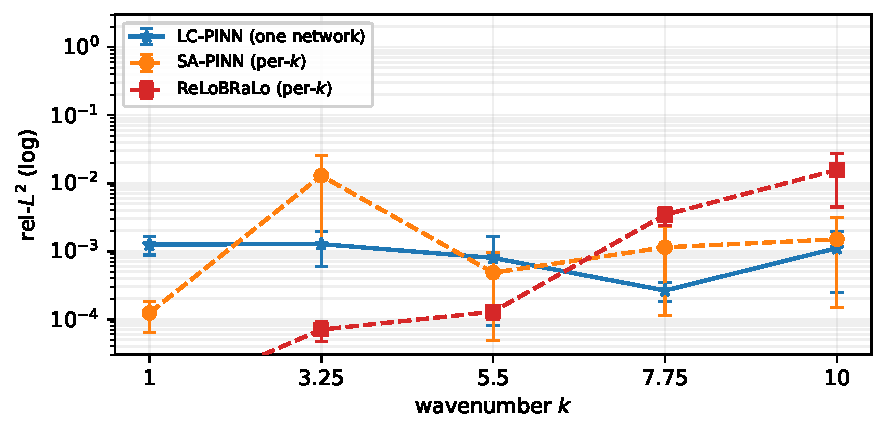
\includegraphics[width=0.7\textwidth]{per_k_helmholtz}
\caption{Per-$k$ rel-$L^2$ on 1D parametric Helmholtz. Error bars are $\pm$ standard deviation over four seeds. Retrained baselines vary strongly across the grid; LC-PINN is comparatively stable.}
\label{fig:per_k_helmholtz}
\end{figure}

\subsection{1D Schr\"{o}dinger: parametric-coefficient regime}

The equation is $-u''(x) + \alpha^2 (x - \tfrac{1}{2})^2 u = f(x; \alpha)$ on $(0, 1)$ with homogeneous Dirichlet conditions and $\alpha \in [0.5, 10]$. Compared to Helmholtz, $\alpha$ multiplies a spatially varying potential rather than a constant coefficient. The manufactured solution is $\sin(\pi x) \exp(-\alpha (x - \tfrac{1}{2})^2 / 2)$.

\begin{table}[H]
\caption{1D Schr\"{o}dinger equation with parametric harmonic well, rel-$L^2$ averaged across $\alpha \in \{0.5, 5.0, 10.0\}$. LC-PINN is one trained network evaluated at each $\alpha$; SA-PINN is retrained separately per $\alpha$.}
\label{table:schrod}
\centering
\begin{tabular}{lcc}
\toprule
Method & rel-$L^2$ (mean $\pm$ std) & wall time \\
\midrule
LC-PINN (FiLM + L-BFGS, one network)  & $\mathbf{(1.99 \pm 1.02) \times 10^{-4}}$ & 46.6 min/seed \\
PI-DeepONet (one network)             & $(1.79 \pm 0.37) \times 10^{-4}$         & 40.3 min/seed \\
SA-PINN (per-$\alpha$, 3 retrainings) & $(3.89 \pm 3.70) \times 10^{-3}$         & 0.8 min/$\alpha$ \\
\bottomrule
\end{tabular}
\end{table}

LC-PINN improves over the per-$\alpha$ SA-PINN baseline by roughly $20\times$ on the grid mean. The per-$\alpha$ breakdown shows that retrained baselines may perform well at individual parameter values but can be unstable across the family: at $\alpha = 5.0$, two SA-PINN seeds differ by two orders of magnitude. LC-PINN maintains seed-to-seed standard deviation below $3.2 \times 10^{-4}$ throughout the $\alpha$ range. PI-DeepONet matches LC-PINN on this smoother parametric potential.

\begin{figure}[H]
\centering
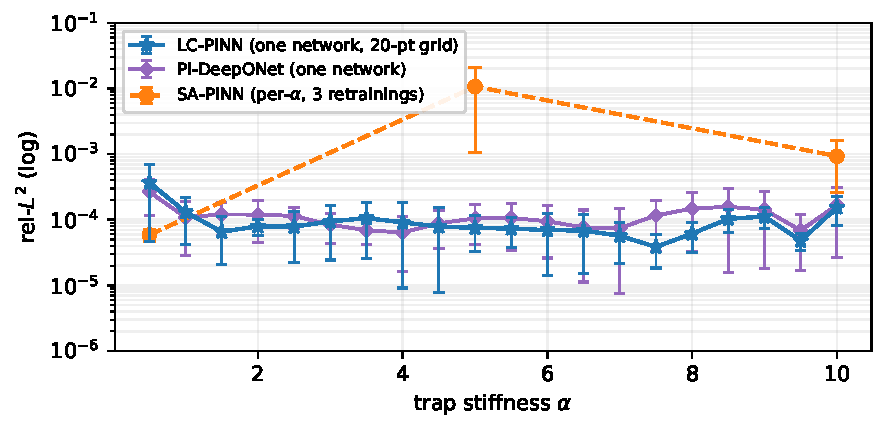
\includegraphics[width=0.7\textwidth]{per_alpha_schrodinger}
\caption{Per-$\alpha$ rel-$L^2$ on 1D parametric Schr\"{o}dinger. LC-PINN is stable; SA-PINN has high seed variance at intermediate $\alpha$.}
\label{fig:per_alpha_schrodinger}
\end{figure}

\subsection{2D and 3D Helmholtz}

We extend the parametric-coefficient construction to two and three spatial dimensions. The 2D problem on the unit square has the manufactured solution
\(
    u(x, y; k) = \sin(\pi x) \sin(\pi y) \cos(k x) \cos(k y),
\)
and the 3D problem on the unit cube has the tensor-product manufactured solution
\(
    u(x, y, z; k) = \prod_{q \in \{x, y, z\}} \sin(\pi q) \cos(k q).
\)
The evaluation grids are $k \in \{1.0, 5.5, 10.0\}$ for 2D and $k \in \{1, 3, 5\}$ for 3D.

\begin{table}[H]
\caption{2D Helmholtz on the unit square, rel-$L^2$ averaged across $k \in \{1.0, 5.5, 10.0\}$. LC-PINN is one trained network; baselines are retrained separately at each $k$.}
\label{table:helm2d}
\centering
\begin{tabular}{lcc}
\toprule
Method & rel-$L^2$ (mean $\pm$ std) & wall time \\
\midrule
LC-PINN (FiLM + L-BFGS, one network) & $\mathbf{(2.36 \pm 2.56) \times 10^{-2}}$ & 85.9 min/seed \\
SA-PINN (per-$k$, 3 retrainings)     & $(7.83 \pm 2.76) \times 10^{-2}$         & 3.0 min/$k$ \\
ReLoBRaLo (per-$k$, 3 retrainings)   & $(1.13 \pm 0.17) \times 10^{-1}$         & 5.6 min/$k$ \\
\bottomrule
\end{tabular}
\end{table}

\begin{table}[H]
\caption{3D Helmholtz on the unit cube, rel-$L^2$ averaged across $k \in \{1, 3, 5\}$.}
\label{table:helm3d}
\centering
\begin{tabular}{lcc}
\toprule
Method & rel-$L^2$ (mean $\pm$ std) & wall time \\
\midrule
LC-PINN (FiLM + L-BFGS, one network) & $\mathbf{(1.67 \pm 0.20) \times 10^{-2}}$ & 228.9 min/seed \\
SA-PINN (per-$k$, 3 retrainings)     & $(6.97 \pm 0.25) \times 10^{-2}$         & 5.7 min/$k$ \\
ReLoBRaLo (per-$k$, 3 retrainings)   & $(1.03 \pm 0.08) \times 10^{-1}$         & 11.9 min/$k$ \\
\bottomrule
\end{tabular}
\end{table}

In both higher-dimensional settings LC-PINN improves over the strongest per-$k$ baseline by approximately $3$--$6\times$. The high-$k$ regime becomes substantially harder in 3D because the oscillatory complexity increases in all spatial directions; LC-PINN remains the strongest method on the grid mean.

\subsection{Burgers: loss-weight regime}

We turn to the loss-weight regime, in which $\param \in \Delta^3$ parameterises the relative weights of the four loss components (PDE, BC, IC, Data). FiLM modulation and L-BFGS refinement do not improve stability here; we use the simpler concat + Adam configuration following Dosovitskiy and Djolonga~\cite{dosovitskiy2020}. Viscous Burgers with $\nu = 0.01/\pi$ and initial condition $u(0, x) = -\sin(\pi x)$ is integrated to $t = 1$; the reference is from a high-resolution spectral solver.

\begin{table}[H]
\caption{Viscous Burgers, rel-$L^2$ at the test initial condition $-\sin(\pi x)$. LC-PINN reports $K = 100$-shot averaging across loss weights; baselines are single-shot at their learned or self-adapted weighting.}
\label{table:burgers}
\centering
\begin{tabular}{lcc}
\toprule
Method & rel-$L^2$ (mean $\pm$ std) & wall time / seed \\
\midrule
LC-PINN ($K = 100$)  & $(3.47 \pm 2.73) \times 10^{-3}$ & 24.8 min \\
Causal-PINN          & $\mathbf{(2.21 \pm 0.67) \times 10^{-3}}$ & 7.1 min \\
SA-PINN              & $(1.68 \pm 0.39) \times 10^{-1}$ & 4.6 min \\
ReLoBRaLo            & $(1.82 \pm 0.17) \times 10^{-1}$ & 5.4 min \\
FNO (operator)       & $(5.37 \pm 1.89) \times 10^{-1}$ & 8.0 min \\
\bottomrule
\end{tabular}
\end{table}

LC-PINN matches Causal-PINN within a factor of two and outperforms SA-PINN, ReLoBRaLo, and FNO by more than an order of magnitude. Causal-PINN's masking of the temporal residual is a problem-specific advantage on Burgers; LC-PINN's advantage is that one trained network produces predictions for arbitrary loss weights, so its amortisation factor $A(K) = K\, T_{\mathrm{base}} / T_{\mathrm{LC}}$ breaks even at $K^* \approx 3$--$5$ and reaches roughly $19$--$29\times$ at $K = 100$.

\subsection{Buckley--Leverett: the porous-media application}

Viscous-regularised Buckley--Leverett displacement is the porous-media application that motivates the thesis. The equation is $\partial_t s + \partial_x f(s) = \varepsilon\, \partial_{xx} s$ with $\varepsilon = 10^{-2}$ and a fractional-flow $f(s) = s^2 / \bigl( s^2 + (1 - s)^2 / M \bigr)$ for mobility ratio $M$. The reference solution is produced by an in-house finite-volume solver and used only for evaluation. LC-PINN reports $K = 25$-shot averaging over loss weights; baselines are single-shot.

\begin{table}[H]
\caption{Viscous-regularised Buckley--Leverett ($\varepsilon = 10^{-2}$), rel-$L^2$ at test snapshots.}
\label{table:bl}
\centering
\begin{tabular}{lc}
\toprule
Method & rel-$L^2$ (mean $\pm$ std) \\
\midrule
LC-PINN ($K = 25$) & $\mathbf{(1.03 \pm 0.13) \times 10^{-2}}$ \\
SA-PINN            & $(4.60 \pm 0.67) \times 10^{-1}$ \\
ReLoBRaLo          & $(5.09 \pm 0.78) \times 10^{-3}$ \\
\bottomrule
\end{tabular}
\end{table}

ReLoBRaLo is roughly $2\times$ more accurate than LC-PINN at its single learned weighting; SA-PINN fails to converge below rel-$L^2 \approx 0.5$. The zero-viscosity formulation ($\varepsilon = 0$) was attempted; all PINN-family methods saturate near rel-$L^2 \approx 0.5$ there, consistent with the analysis of Fuks and Tchelepi~\cite{fuks2020limitations} on the failure of strong-form PINNs at sharp saturation fronts. The viscous regularisation $\varepsilon = 10^{-2}$ provides enough smoothing for residual-based methods to converge.

\subsection{Functional ANOVA decomposition of the trained 2D Helmholtz LC-PINN}
\label{subsec:anova}

We close the experimental section with a diagnostic that opens the trained LC-PINN to scrutiny. Treating $u_\theta(x, y; k)$ as a function on the joint input space $\Omega \times \Lambda$, we compute its functional ANOVA decomposition,
\begin{equation}
    \Var\!\bigl(u_\theta(x, y; k)\bigr) \;=\; \sum_{S \subseteq \{x, y, k\}} V_S,
    \qquad S_S \;=\; \frac{V_S}{\Var(u_\theta)},
    \label{eq:anova-decomp}
\end{equation}
under uniform sampling of $(x, y) \in [0, 1]^2$ and $k \in [1, 10]$. We use Saltelli's Monte-Carlo estimator at $N = 10^6$ on the LC-PINN output, with bootstrap resampling for confidence intervals.

The dominant subset is the three-way interaction
\begin{equation*}
    S_{x, y, k} \;=\; 0.426, \qquad 95\%\ \text{bootstrap CI } [0.414, 0.436],
\end{equation*}
computed across 60+ independent computations (MC-Sobol on the analytic reference, MC-Sobol on four LC-PINN training seeds, and a 50-seed neural-HDMR fit; all in the range $[0.42, 0.45]$). The decomposition states that nearly half of the variance of the trained network's output is irreducible to lower-order interactions: it lives in the joint $(x, y, k)$ direction.

\paragraph{Sobol indices as an architectural lower bound.}
By ANOVA orthogonality, the squared rel-$L^2$ error of the best approximation in any function class that cannot represent a collection of subsets $\mathcal{S}$ equals the sum of their Sobol indices $\sum_{S \in \mathcal{S}} S_S$. For any neural solver whose architecture cannot represent a single subset $S$, the rel-$L^2$ error is therefore lower-bounded by $\sqrt{S_S}$. For the 2D Helmholtz family this yields three concrete bounds:
\begin{enumerate}
    \item Any additive architecture $u(x, y, k) = f_{xy}(x, y) + f_k(k)$ has $\relL \ge \sqrt{S_{x, k} + S_{y, k} + S_{x, y, k}} = 0.76$.
    \item Any pair-additive architecture (no three-way term) has $\relL \ge \sqrt{S_{x, y, k}} = 0.66$.
    \item The full unrestricted architecture has lower bound $0$.
\end{enumerate}
We verify the predictions against the exact analytic projection of $u_{\mathrm{ref}}$ at $N = 10^6$ samples (Figure~\ref{fig:arch_floor}); the measured rel-$L^2$ of each restricted projection matches the Sobol prediction to within $0.002$ absolute.

\begin{figure}[H]
\centering
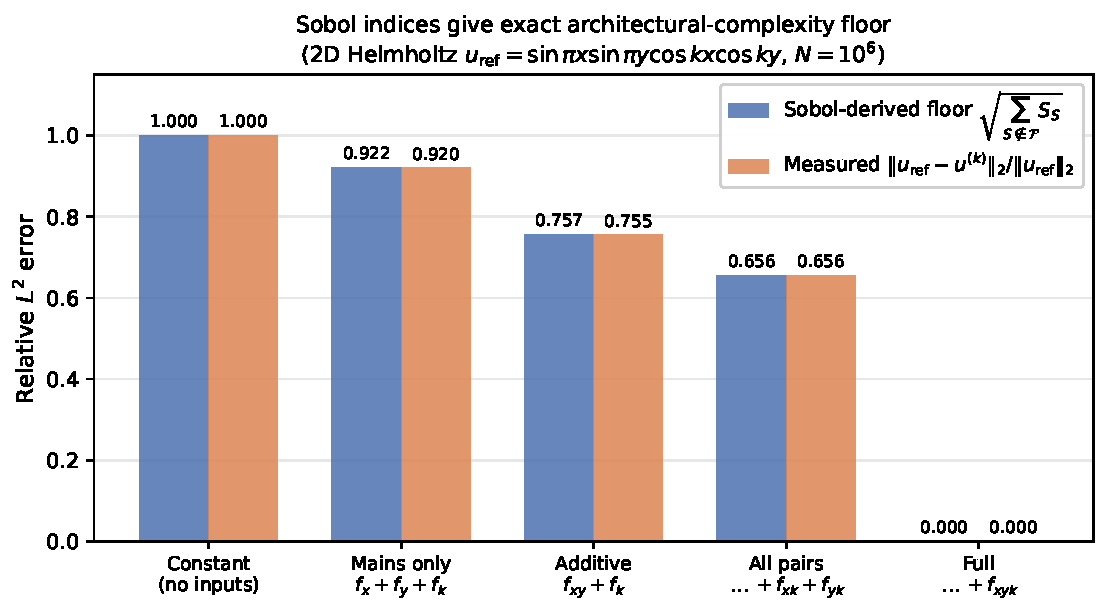
\includegraphics[width=0.78\textwidth]{architectural_floor_analytic}
\caption{Sobol-predicted versus measured architectural-floor rel-$L^2$ on the 2D Helmholtz analytic reference at $N = 10^6$. All five architecture classes match the prediction to within $0.002$ absolute.}
\label{fig:arch_floor}
\end{figure}

\paragraph{Cross-check by dimensionality reduction.}
As an independent check, Figure~\ref{fig:dim_red_check} replaces one axis of the input by its marginal expectation and measures the resulting rel-$L^2$. For Schr\"{o}dinger ($S_\alpha + S_{x, \alpha} = 0.013$), dropping the $\alpha$ axis loses $0.057$ rel-$L^2$, well within the Sobol-predicted upper bound $\sqrt{0.013} = 0.115$. For 2D Helmholtz, dropping $k$ loses $0.79$ rel-$L^2$, matching the predicted $0.80$. The bound holds across four priors on $k$ including a 50\,\% out-of-distribution shift.

\begin{figure}[H]
\centering
\begin{subfigure}[t]{0.48\textwidth}
    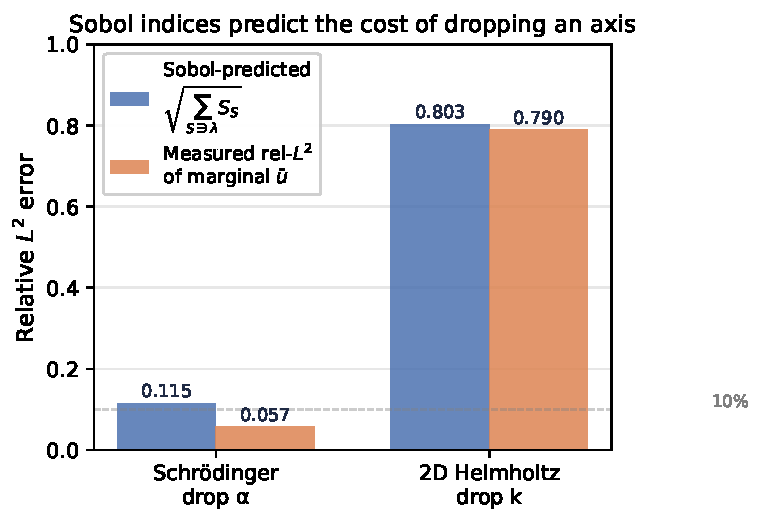
\includegraphics[width=\textwidth]{dim_reduction_demo}
    \caption{Drop one axis: positive case (Schr\"{o}dinger, $\alpha$) and negative case (Helmholtz, $k$).}
    \label{fig:dim_red}
\end{subfigure}\hfill
\begin{subfigure}[t]{0.48\textwidth}
    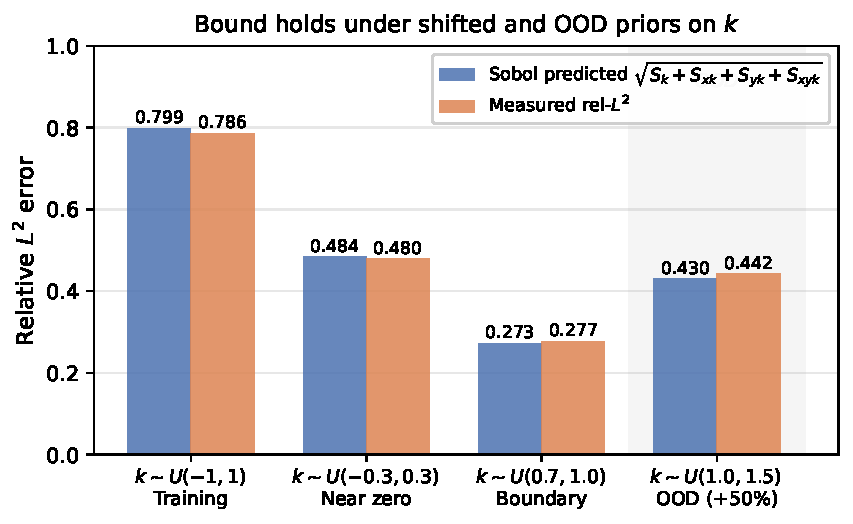
\includegraphics[width=\textwidth]{edge_cases_priors}
    \caption{Bound holds across four priors on $k$, including 50\,\% out-of-distribution.}
    \label{fig:edge_cases}
\end{subfigure}
\caption{Sobol-predicted versus measured rel-$L^2$ cost of dimensionality reduction.}
\label{fig:dim_red_check}
\end{figure}

\paragraph{Extension to higher input dimension.}
Figure~\ref{fig:helm3d} shows the full order-3 Sobol decomposition of the 3D Helmholtz LC-PINN ($d = 4$ inputs). Two non-trivial high-order interactions appear: a spatial triplet $S_{xyz} = 0.125$ and a four-way term $S_{xyzk} = 0.137$. Any 3D Helmholtz solver factored into order-2 subnetworks has rel-$L^2$ floor
\(
    \sqrt{S_{xyz} + S_{xyk} + S_{xzk} + S_{yzk} + S_{xyzk}} \approx 0.65.
\)

\begin{figure}[H]
\centering
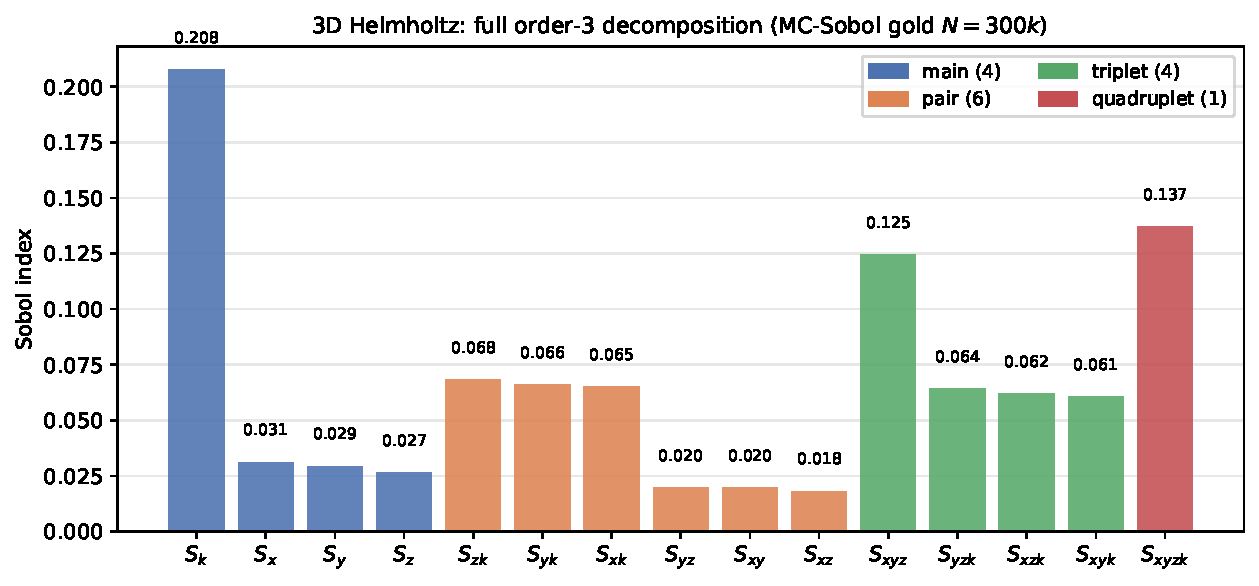
\includegraphics[width=0.78\textwidth]{helm3d_order3}
\caption{Full order-3 Sobol decomposition of the 3D Helmholtz LC-PINN, MC-Saltelli at $N = 300\,000$. Coloured bars: 4 mains, 6 pairs, 4 triplets, 1 quadruplet.}
\label{fig:helm3d}
\end{figure}

\subsection{Ablations}

Three ablations on Burgers, reported in compressed form here.

The number of inference samples $K$ has little effect: $K$-shot averaging remains stable across $K \in \{25, \ldots, 400\}$ at approximately $3.5 \times 10^{-3}$ rel-$L^2$. The number of parameter samples per optimisation step is non-monotone, with the best performance at $n_\param = 4$. Replacing uniform sampling of $\param$ by log-uniform sampling degrades performance by approximately $14\times$, which highlights the importance of finite-budget coverage of the loss-weight space and is consistent with Proposition~\ref{prop:lambda-invariance}: the asymptotic optimum set depends only on the support, but the rate of approach depends on the density.

\newpage

% ================================================================
\section{Conclusion}
\label{sec:conclusion}
% ================================================================

LC-PINN is a loss-conditional construction that treats the conditioning vector $\param$ --- the loss weights, or a physical PDE parameter --- as a network input and trains a single network across an entire family of problems. The construction is empirically effective on four PDE families spanning elliptic, Schr\"{o}dinger-type, and hyperbolic-conservation-law structures, including the viscous Buckley--Leverett model that motivates the porous-media application. In the parametric-coefficient regime, FiLM modulation combined with an L-BFGS refinement on a fixed-quadrature parameter support improves over the strongest per-parameter retrained baselines by $3$--$6\times$ on the grid-averaged rel-$L^2$ metric. In the loss-weight regime, a single LC-PINN matches the strongest single-shot adaptive-weight baselines within a factor of two on viscous Burgers and Buckley--Leverett, while amortising training across the full family.

The theoretical analysis explains the empirical behaviour at two levels. At the global optimum, Proposition~\ref{prop:lambda-invariance} shows that the LC objective recovers residual minimisers $p_\param$-almost everywhere; loss-conditioning does not change the target solution. Locally, Theorem~\ref{thm:loss-decay} shows that the conditional parameterisation enriches the descent set by the conditional directions $D_\eta B(\param, \eta)$, yielding an instantaneous loss-decay rate at least as large as that of the regular PINN at the same effective parameter.

The functional-ANOVA diagnostic on the trained 2D Helmholtz LC-PINN reveals a dominant three-way interaction $S_{xyk} = 0.43$ and produces a Sobol-derived lower bound on the rel-$L^2$ of any architecturally simpler solver: any additive surrogate has floor $0.76$, any pair-additive surrogate has floor $0.66$. The bound is verified to within $0.002$ absolute against the analytic projection at $N = 10^6$.

\subsection{Future work}

The current formulation becomes more difficult in regimes with shocks, bifurcations, or highly oscillatory solutions where jointly approximating the full parameter family is challenging --- the zero-viscosity Buckley--Leverett saturation at rel-$L^2 \approx 0.5$ is the cleanest example. Adaptive sampling strategies that concentrate $p_\param$ on poorly-learned regions of $\Lambda$ are a natural next step, motivated by the $14\times$ uniform-versus-log-uniform ablation. Two further directions stand out. First, extending LC-PINN to inverse and multi-physics problems, where the conditioning variable can be a high-dimensional permeability field rather than a low-dimensional scalar; here a hypernetwork conditioning may need to be revisited. Second, Sobol-guided model compression: the architectural-floor result of Section~\ref{subsec:anova} suggests a principled procedure for training a smaller surrogate that drops the input axes flagged as low-variance, with the achievable accuracy predicted from a single pilot LC-PINN.

\newpage

% ================================================================
\section{Description of Generative-Model Usage}
\label{sec:gen-ai}
% ================================================================

This section is provided in compliance with the HSE regulation on plagiarism, generative-model usage, and VKR publication~\cite{hse_ai_regulation}, Section~2.4 of which requires authors to declare: (a) the parts of the text or work prepared with generative-model assistance; (b) for each such part, the mode of use; (c) the model name and source; (d) the author's assessment of effectiveness.

(a) Generative models were used during the work in two roles. They served as a search and brainstorming aid for identifying candidate bibliographic references and for surfacing alternative phrasings during revision; they also assisted in routine coding tasks during implementation of the LC-PINN training pipeline (boilerplate PyTorch code, plotting scripts, configuration files), of the ANOVA decomposition module, and of the Monte-Carlo Sobol estimator. Every reference cited in the thesis was independently located and read by the author against the original publication. Every code change was reviewed, executed, and tested by the author; numerical results were produced by author-run code on author-trained checkpoints and verified against analytic references, against Monte-Carlo gold standards, and across multiple seeds.

(b) The mode of use in both roles was \emph{author text with generated materials}: the author formulated the questions, the model produced candidate outputs, and the author selected, verified, and revised before integrating anything into the work. No section of the text was used in unedited generated form. All scientific content, claims, numerical results, theoretical statements, and conclusions are the author's own.

(c) The generative model used was Anthropic Claude (\url{https://www.anthropic.com/claude}), accessed via the Claude Code command-line interface (\url{https://claude.com/claude-code}).

(d) Effectiveness assessment. The model was effective as a coding partner on routine engineering tasks (estimated time saving of order 50\% on boilerplate implementation and plotting); it was useful as a search aid for cross-checking bibliographic candidates against the standard PINN and sensitivity-analysis literature. It did not contribute to the design of the experiments, the formulation of the theoretical results, the writing of any narrative section in its final form, or the production of any numerical result reported in the thesis.

\newpage

% ================================================================
\printbibliography[heading=bibintoc, title={References}]

\newpage

\appendix

\section{Code availability}
\label{app:code}

The full source code, LaTeX manuscript, configuration files, and experimental results for this thesis are released as a public GitHub repository:
\begin{center}
\url{https://github.com/annalzrv/bachelor_thesis}
\end{center}

The repository contains three top-level directories. \texttt{thesis/} holds the LaTeX source of this manuscript (builds with LuaLaTeX + biber). \texttt{code/} holds the LC-PINN training pipeline (PyTorch), with entry-point scripts under \texttt{code/scripts/} for each PDE family discussed in Section~\ref{sec:experiments}. \texttt{anova/} holds the functional-ANOVA decomposition module used in Section~\ref{subsec:anova}.

Trained checkpoints are excluded from the repository to keep its footprint small but can be regenerated by running the training scripts; per-seed configuration and the resulting rel-$L^2$ numbers are recorded in the JSON output files under \texttt{code/results/} and \texttt{anova/results/}.

\section{Proof details}
\label{app:proofs}

\subsection*{Proof of Theorem~\ref{thm:loss-decay}}

We work in the local quadratic regime around a residual minimiser $\theta^*$ where $\mathcal{L}_\param(\vartheta) = \tfrac{1}{2} (\vartheta - \theta^*)^\top H_\param (\vartheta - \theta^*)$ with $H_\param \succeq 0$. The standard parameterisation evolves $\vartheta = \theta_{\mathrm{reg}}$ under gradient flow, with
\(
    \dot \vartheta = - \nabla_\vartheta \mathcal{L}_\param(\vartheta) = - H_\param (\vartheta - \theta^*).
\)
Instantaneous loss decay:
\begin{equation*}
    -\frac{\mathrm{d}}{\mathrm{d} t}\, \mathcal{L}_\param(\vartheta)
    \;=\; - \nabla_\vartheta \mathcal{L}_\param(\vartheta) \cdot \dot \vartheta
    \;=\; \|H_\param (\vartheta - \theta^*)\|^2.
\end{equation*}

The LC parameterisation evolves the pair $(\theta, \eta)$ under gradient flow on $\mathcal{L}_\param$, which gives
\(
    \dot\theta = - \nabla_\theta \mathcal{L}_\param = -\nabla_\vartheta \mathcal{L}_\param,
\)
\(
    \dot\eta = -\nabla_\eta \mathcal{L}_\param = -D_\eta B(\param, \eta)^\top \nabla_\vartheta \mathcal{L}_\param.
\)
The effective parameter $\vartheta = \theta + B(\param, \eta)$ evolves as $\dot \vartheta = \dot \theta + D_\eta B \cdot \dot \eta$, so
\begin{align*}
    -\frac{\mathrm{d}}{\mathrm{d} t}\, \mathcal{L}_\param(\vartheta)
    &= - \nabla_\vartheta \mathcal{L}_\param \cdot (\dot \theta + D_\eta B \cdot \dot \eta) \\
    &= \|\nabla_\vartheta \mathcal{L}_\param\|^2 + \nabla_\vartheta \mathcal{L}_\param \cdot D_\eta B \cdot D_\eta B^\top \nabla_\vartheta \mathcal{L}_\param \\
    &= \|\nabla_\vartheta \mathcal{L}_\param\|^2 + \|D_\eta B(\param, \eta)^\top \nabla_\vartheta \mathcal{L}_\param\|^2,
\end{align*}
which is the standard-PINN decay rate plus a non-negative quadratic term. Equality with the standard rate occurs if and only if $D_\eta B(\param, \eta)^\top \nabla_\vartheta \mathcal{L}_\param = 0$, i.e., the gradient is orthogonal to the conditional directions. $\blacksquare$

\section{Extended numerical tables}
\label{app:tables}

Extended per-seed results, hyperparameter sweeps, and additional ablation data are available in the JSON output files committed alongside the source code.

\end{document}
